\section{Modeling}\label{sec:model}


Section outline:

\begin{enumerate}
\item \cmark section intro
\item \cmark fix order from simplest to most complex
\item Description of DCE and parameter estimation  
\item Description of auto ARIMA 
\subitem (this should be limited and explain it is meant to be out of the box) point at the paper for auto arima for more details.
\item \cmark Description of the two naive methods (random walk and mean), make sure to explain that these methods are naive and simple but not necessarily bad.
\item\cmark Add a section talking about evaluation methods i.e., MASE, this text is currently written and just sitting at the beginning of the results. 

\end{enumerate}

In this section we describe the four different forecasting schema used in this study. In Section \ref{sec:simple} we outline two primitive strategies which often out perform sophisticated prediction strategies in the case of highly complex signals. In Section \ref{sec:arima} we describe Autoregressive integrated moving-average (ARIMA) a commonly used linear forecasting scheme. In Section \ref{sec:lma} we describe a simple nonlinear deterministic forecasting scheme, Lorenz Method of Analogous (LMA) for capturing and exploiting nonlinear dynamics present in a time series. And finally in Section \ref{sec:accuracy} we discuss the error metric we use to evaluate each models predictive accuracy.



\subsection{Primitive Strategies to combat complexity: Random Walk and \naive}\label{sec:simple}
In this section we cover two very simple forecast models: Random Walk and \naive. With a Random Walk predictor to forecast at time $i$ we simply use the last observed measurement: $$p_i = X_{i-1,obs}$$. The \naive prediction strategy is to forecast the rolling average up to that point. i.e., the prediction $p_i$ is simply the average of all observed points up to that point: $$p_i = \sum_{j=1}^{i-1}\frac{X_{j,obs}}{i-1}$$.

While both of these methods are simplistic they are not without merit. When time series possess very little predictive structure,i.e., they exist on the very top of the complexity spectrum these two methods can sometimes be \emph{on-average} very good choices for a forecasting method, as we will see in our results. An example is forecasting currency exchange rates. In \cite{rwMeese,rwCCE} the authors show that various econometric techniques and prediction models fail to consistently outperform Random Walk predictions in forecasting various exchange rates. This is the case because these signals are volatile, noisy and possess very little information structure but they don't \emph{on-average} vary a great deal. That is the day-to-day exchange rates \emph{on-average} don't vary very much so guessing the last known exchange rate is often a very good approximation to the new exchange rate. [[Not a huge fan of this wording.]] The Na\"ive forecasting scheme can be a great prediction strategy if the time series has very little forward information structure, adheres to a unimodal distribution and has very little variance. In this circumstance, forecasting the mean will on average get you in the ball park of the forecast without taking into account the lack of structure. The \naive forecasting scheme can be thought of as a filtering mechanism which compresses a signal onto a single point, effectively filtering out both complexity and structure. However, if very little predictive structure is present in a signal then this filtering mechanism effectively mitigates the complexity.     

While the simplicity of these methods is advantageous when a signal is mostly complexity, i.e., that is the time series exists on the high side of the complexity spectrum, the methods can be inconsistent in their forecasting ability as a consequence of not being dynamic or taking into account the distribution or structure of the time series. Both of these methods fail spectacularly in two specific circumstances that lie on the fringes of their strengths. Fortunately, they somewhat parallel each other, i.e., the weakness of Random Walk and \naive are covered by the other primitive method. The situation in which Random Walk fails is when a time series changes drastically on a regular basis. The simplest example of this would be a period 2 time series which alternated between 0 and 1 at each time step. At every time step Random Walk would preciesly predict out of phase, and as a result would accrue an error of 1 at every time step ($|p_i-X_{i,obs}|=1$. In comparison, the \naive method would forecast 0.5 at each time step and would thus accrue and error of 0.5 at every step. So on-average \naive would do twice as well as Random Walk, and as you could imagine a dynamic method would captured this periodicity  and exploited this predictive structure could do much much better, such a method is introduced in Section \ref{sec:lma}. 

The \naive forecast fails when you have a signal which shifts between two or more regimes on a regular basis and the regimes are separated by a significant amount. In this case the \naive forecast will predict between the multiple regimes at every time step eventually accruing massive error. To see how Random Walk can cover this weakness imagine a time series which switches between more than one regime but stays in each regime for several time steps, this behaviour can be seen in some portions of the \svd trace seen in Figure \ref{fig:ts}. Random walk in this case could react to the regime shift within one time step, switch to the new Regime and begin forecasting nicely, where as \naive would just continue to predict between the modes of the multimodal distribution resulting in poor forecasting accuracy all of the time. 

So clearly these primitive methods have their downfalls, but it is important to keep in mind that when a time series exists on the top of the complexity spectrum they have little predictive structure to exploit and often a primitive method like Random Walk or \naive will consistently out perform methods which rely on predictive structure. This is explored further in Section \ref{sec:accuracy} and \ref{sec:results}


\subsection{Linear Forecasting: Seasonal Autoregressive-integrated-moving average(ARIMA)}\label{sec:arima}
\begin{enumerate}
\item\cmark introduce method abstractly and practically, common method basically fitting a hyperplane to data removing seasonality and filtering for noise
\item\cmark define rigorously, all the backshift operator garbage

$$\Phi(B^m)\phi(B)(1-B^m)^D(1-B)^dX_i = c + \Theta(B^m)\theta(B)\epsilon_i$$

$$B^mX_i  = X_{i-m}$$
\item\cmark discuss that this method needs linear structure to work correctly
\item \cmark maybe talk about converging to zero and limits on prediction horizon
\end{enumerate}

For this \cite{davislinearts}

When there is evidence a generating process exhibits predictive structure an obvious strategy would be to fit a hyperplane to the dataset and then use this hyperplane to forecast new data points. This is a very old technique stemming back to Yule in 1927\cite{weigend93} with his invention of autoregressive forecasting, which forecasts the next time step through a weighted average of the past $p$ time-steps, i.e., $$p_i = \phi(B)X_{i,obs}.$$ Here $\phi(B)$ is a polynomial of degree $p$ and $B$ is the backshift operator, i.e., $$B^mX_i  = X_{i-m,obs}.$$
To improve this method further, especially in the presence of noisy data would be to allow for some wiggle room by adding a moving average of white noise to the model: $\theta(B)\epsilon_i$, where $\theta(B)$ is a polynomial of degree $q$ and $\{\epsilon_i\}\sim WN(0,\sigma^2)$. Finally if there is evidence of non-stationarity an initial differencing (integrated) is applied as an attempt to remove that non-stationarity: $(1-B^d)X_i$. Combining these three give us a nonseasonal  ARIMA$(p,d,q)$ model:  $$\phi(B)(1-B)^dX_i = \theta(B)\epsilon_i.$$ Where $p$, $d$ and $q$ correspond to the orders of the autoregressive, integrated and moving average models respectively. If periodic structure is present a seasonal ARIMA$(p,d,q)(P,D,Q)_m$ is often used and is defined by:$$\Phi(B^m)\phi(B)(1-B^m)^D(1-B)^dX_i = \Theta(B^m)\theta(B)\epsilon_i.$$ Here $\Phi$ and $\Theta$ are polynomials of degree P and Q respectively, and $m$ is the seasonal frequency. Forecasting is then done in two steps, first the integrated step is performed to remove non-stationarity. $$\hat{X_i} = (1-B^m)^D(1-B)^d X_{i,obs}$$. Then forecasts are made by evaluating $$\Phi(B^m)\phi(B)\hat{X_i} = \Theta(B^m)\theta(B)\epsilon_i.$$

There is a vast amount of theory and literature on constructing, fitting and forecasting with this class of models. However, this is not the focus of this paper and  we refer the reader to \cite{davislinearts} for an in-depth exploration. In this paper, we intend to explore how predictive accuracy of several different forecasting schema correlates with signal complexity. As such, we use ARIMA$(p,d,q)(P,D,Q)_m$ (or simply ARIMA) models as an out of the box black box linear forecasting scheme. To do this we use an automated fitting and forecasting techniques described in \cite{autoARIMA}. This technique automatically selects model and differencing orders: $p, d, q, P, D, Q$ and $m$ as well as fitting the corresponding polynomials to the time series. Hyndman and Khandakar use unit root tests to select differencing orders, $d$ and $D$. In particular, they use a combination of  
KPSS unit-root tests \cite{KPSSunit} and their own extension of Canova-Hansen test \cite{Canova1995}. To do model order selection they use the Akaike information criterion (AIC) \cite{akaike1974} conditioned on the maximized likelihood of the  model fitted to the differenced data, $(1-B^m)^D(1-B)^d X_{i,obs}$ \cite{autoARIMA}. For more detail on this fitting process see \cite{autoARIMA}.

ARIMA forecasting is a time tested modelling process which uses a global linear fit and adjustments for seasonality, non-stationarity and noise. If a generating process fits into one of these categories then this model is a great short term predictor. If information is instead being transmitted in a nonlinear way this global linear fit falls apart. One other weakness of this method is that if long prediction horizons are used the forecast is guaranteed to converge to the mean after some number of predictions. For this reason, we limit all methods to doing multiple 1-step predictions as to not handicap this method. 

\subsection{Nonlinear Forecasting: Lorenz Method of Analogues (LMA)}\label{sec:lma}

When a generating process exhibits deterministic predictive nonlinear structure a common approach is to reconstruct the generating processes dynamics using a technique called delay-coordinate embedding and then use the geometric structure of this reconstruction as a proxy for the information transmission process of the underlying process to predict the future. In this section we discuss the theory and implementation of this forecasting scheme. 


 \subsubsection{Reconstructing hidden dynamics}



Delay-coordinate embedding allows one to reconstruct a system's full
state-space dynamics from a \emph{single} scalar time-series
measurement---provided that some conditions hold regarding that data.
Specifically, if the underlying dynamics and the measurement
function---the mapping from the unknown state vector $\vec{X}$ to the
scalar value $x$ that one is measuring---are both smooth and generic,
Takens~\cite{takens} formally proves that the delay-coordinate map
\[
F(\tau,m)(X) = ([X_{i+\tau,obs} ~ X_{i+\tau,obs} ~ \dots ~X_{i+m\tau,obs}])
\]
from a $d$-dimensional smooth compact manifold $M$ to $\mathbb{R}^{2d+1}$,
where $t$ is time, is a diffeomorphism on $M$---in other words, that
the reconstructed dynamics and the true (hidden) dynamics have the
same topology.

This is an extremely powerful result: among other things, it means
that one can build a formal model of the full system dynamics without
measuring (or even knowing) every one of its state variables.  This is
the foundation of this modeling approach.
The first step in the process is to estimate values for the two free
parameters in the delay-coordinate map: the delay $\tau$ and the
dimension $m$.  We follow standard procedures for this, choosing the
first minimum in the average mutual information as an estimate of
$\tau$ \cite{fraser-swinney} and using the false-near(est) neighbor
method of \cite{KBA92}.  A
plot of the data from Figure~\ref{fig:ipc}, embedded following this
procedure, is shown in Figure~\ref{fig:embedding}.


 \begin{figure}
   \centering
     \includegraphics[width=\textwidth]{figs/colipc3d.png}
     \caption{[[{\color{red}Joshua:Perhaps add a similar graphic of \gcc to show contrast}{\color{green}agreed I will work on this}]]A 3D projection of a delay-coordinate embedding of the trace
 from Figure~\ref{fig:ipc} with a delay ($\tau$) of 100,000 instructions.
 }
 \label{fig:embedding}
 \end{figure}


%% can cut for space if need be:
The coordinates of each point on this plot are differently delayed
elements of the \col instructions per cycle time series
$X_{i,obs}$: that is, $X_{i,obs}$ on the first axis, $X_{i+\tau,obs}$ on the second,
$X_{i+2\tau,obs}$ on the third, and so on.
Structure in these kinds of plots---clearly visible in
Figure~\ref{fig:embedding}---is an indication of
determinism%\footnote{A deeper analysis of
  %Figure~\ref{fig:embedding}---as alluded to on the previous
  %page---supports that diagnosis, confirming the presence of a chaotic
  %attractor in these cache-miss dynamics, with largest Lyapunov
  %exponent $\lambda_1 = 8000 \pm 200$ instructions, embedded in a
  %12-dimensional reconstruction space \cite{mytkowicz09}.}
  .  That structure can be used to build a forecast model.
 \subsubsection{LMA: Using dynamics in forecasting}

Given a nonlinear model of a deterministic dynamical system in the
form of a delay-coordinate embedding like Figure~\ref{fig:embedding},
one can build deterministic forecast algorithms by capturing and
exploiting the geometry of the embedding.  Many techniques have been
developed by the dynamical systems community for this purpose
(e.g.,~\cite{weigend-book,casdagli-eubank92,Smith199250}).  Perhaps the most straightforward
is the ``Lorenz method of analogues'' (LMA), which is essentially
nearest-neighbor prediction in the embedded state
space~\cite{lorenz-analogues}.  Even this simple algorithm---which
builds predictions by finding the nearest neighbor in the embedded
space of the given point, then taking that neighbor's path as the
forecast---works quite well on the trace in Figure~\ref{fig:ipc}, as
shown in Figure~\ref{fig:lmacol}.
%
\begin{figure}[htbp]
  \centering
   \includegraphics[width=\textwidth]{figs/colPredShortTS}
    \caption{A forecast of the last 4,000 points of the signal in
      Figure~\ref{fig:ipc} using an LMA-based strategy on the
      embedding in Figure~\ref{fig:embedding}.  Red circles and blue
      $\times$s are the true and predicted values, respectively;
      vertical bars show where these values differ.}
\label{fig:lmacol}
\end{figure}
%
On the other hand, if we use the same approach to forecast the
processor load (ipc) of the \gcc program from the SPEC cpu2006 benchmark suite, the
prediction is far less accurate; see Figure~\ref{fig:lmagcc}.

\begin{figure}[htbp]
  \centering
    \includegraphics[width=\textwidth]{figs/colPredShortTS}
     \caption{{\color{red} [[actually need to generate this figure]]}An LMA-based forecast of the last 4,000 points of a
       processor-load performance trace from the \gcc
       benchmark.  Red circles and blue $\times$s are the true and
       predicted values, respectively; vertical bars show where these
       values differ.}
\label{fig:lmagcc}
\end{figure}

This gets at the utility of the contribution of this paper: If these traces both come from deterministic
systems---computers---then why are they not equally predictable?  Our
conjecture is that while they come from similar systems \gcc produces processor load traces on the top of the complexity spectrum whereas \col produces processor loads with complexity in the mid to low region of the complexity spectrum. If this is the case then \gcc might be much better predicted using a method like Random Walk or \naive which can effectively predict in the presence of complexity. This is explored more rigorously in the results Section of this paper (Section \ref{sec:results}. So that we don't have to compare the forecast accuarcy by visual comparing the predictions we calculate a figure of merit to compare the predictions. 

%% [[If space: Add a segue sentence: next section uses permutation
%% entropy to explore that conjecture.]]

%\subsection{Comparing Prediction Accuracy}





\subsection{Prediction Accuracy: Mean Absolute Scaled Error (MASE)}
\label{sec:accuracy}

\begin{figure}[htbp]
  \centering
      \begin{subfigure}{0.49\textwidth}
    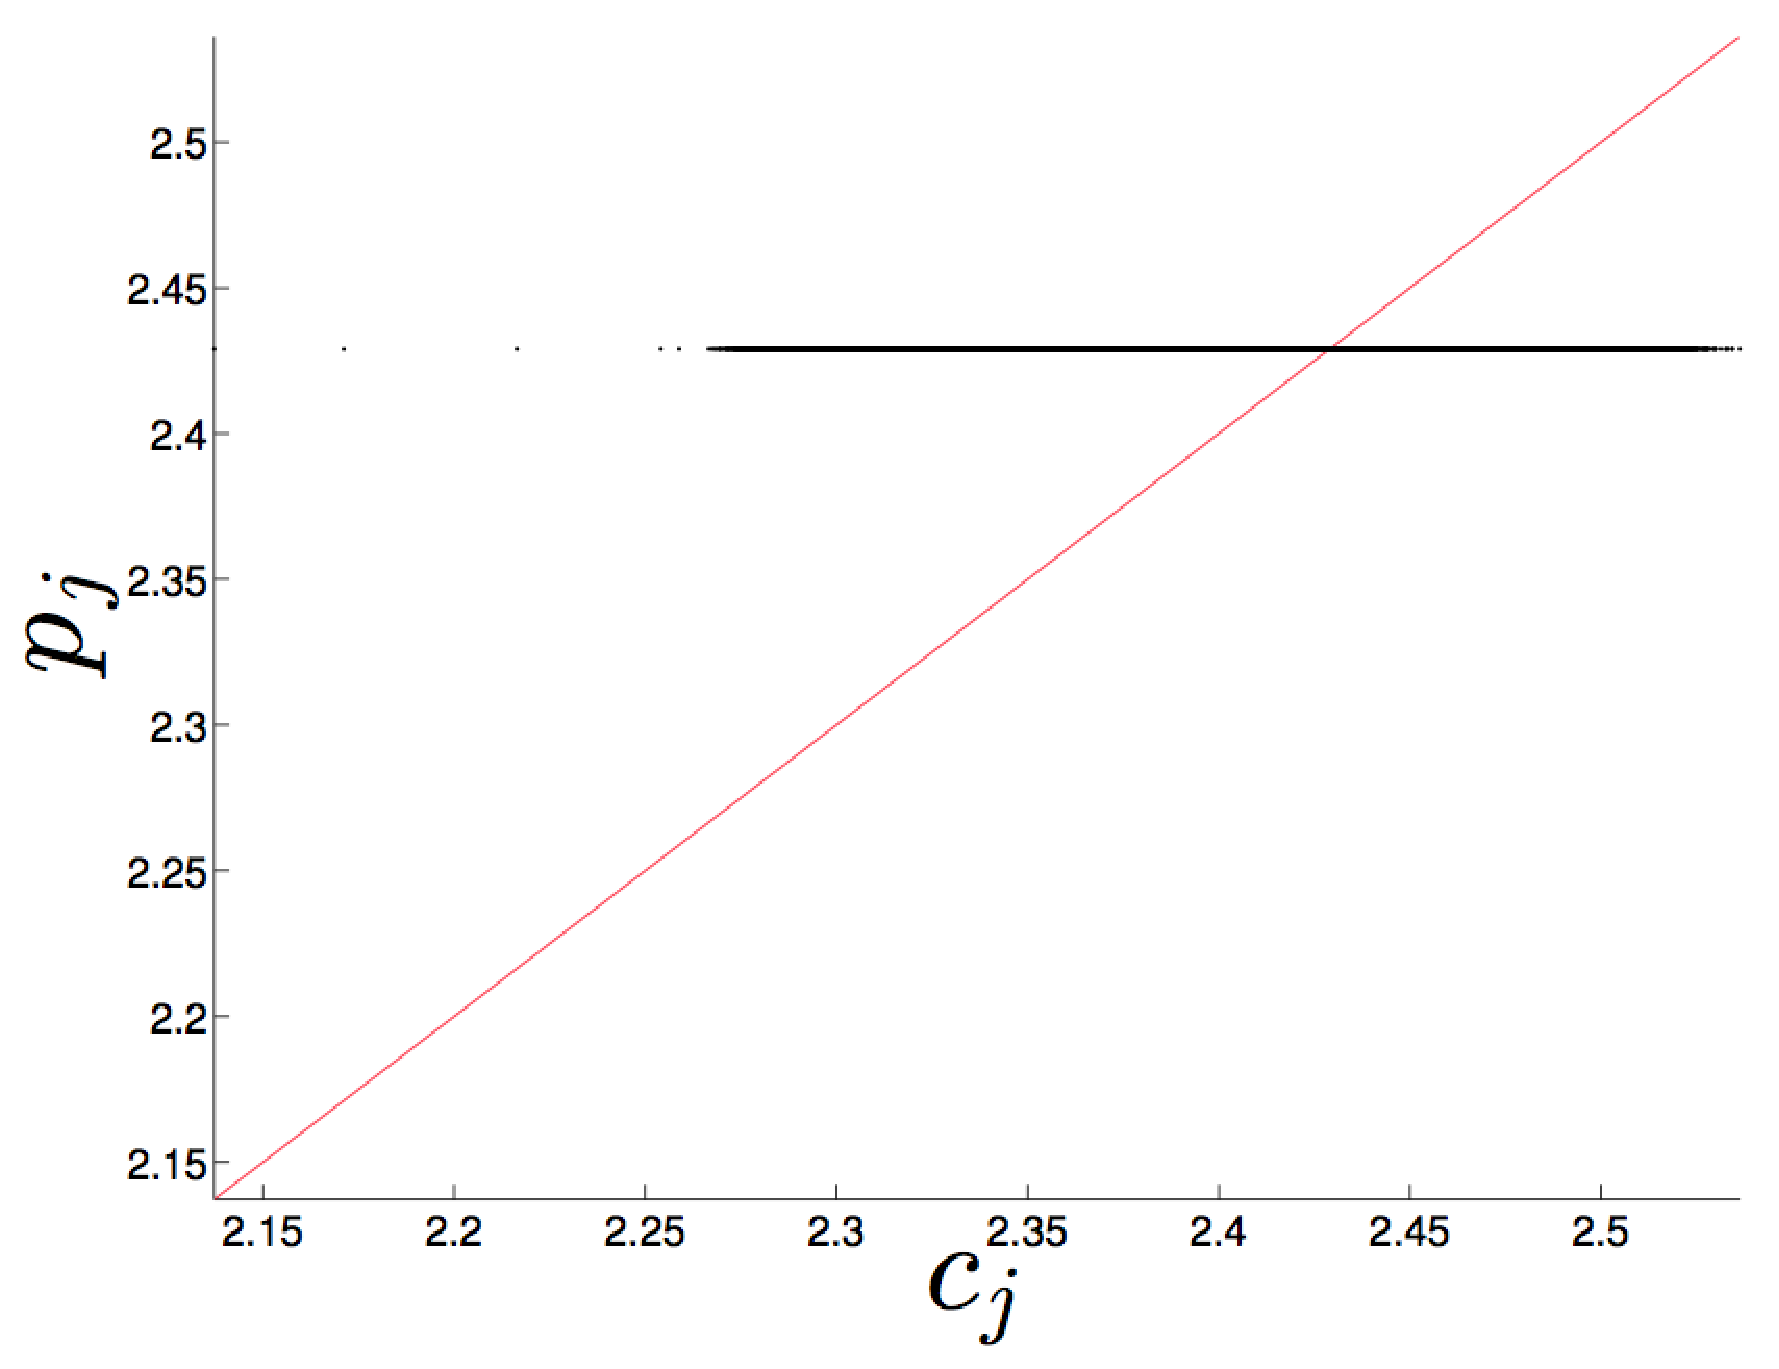
\includegraphics[width=\textwidth]{figs/colMeanForecast}
    \caption{\col na\"ive }
    \label{fig:gccMEAN}
  \end{subfigure}%
   \begin{subfigure}{0.49\textwidth}
    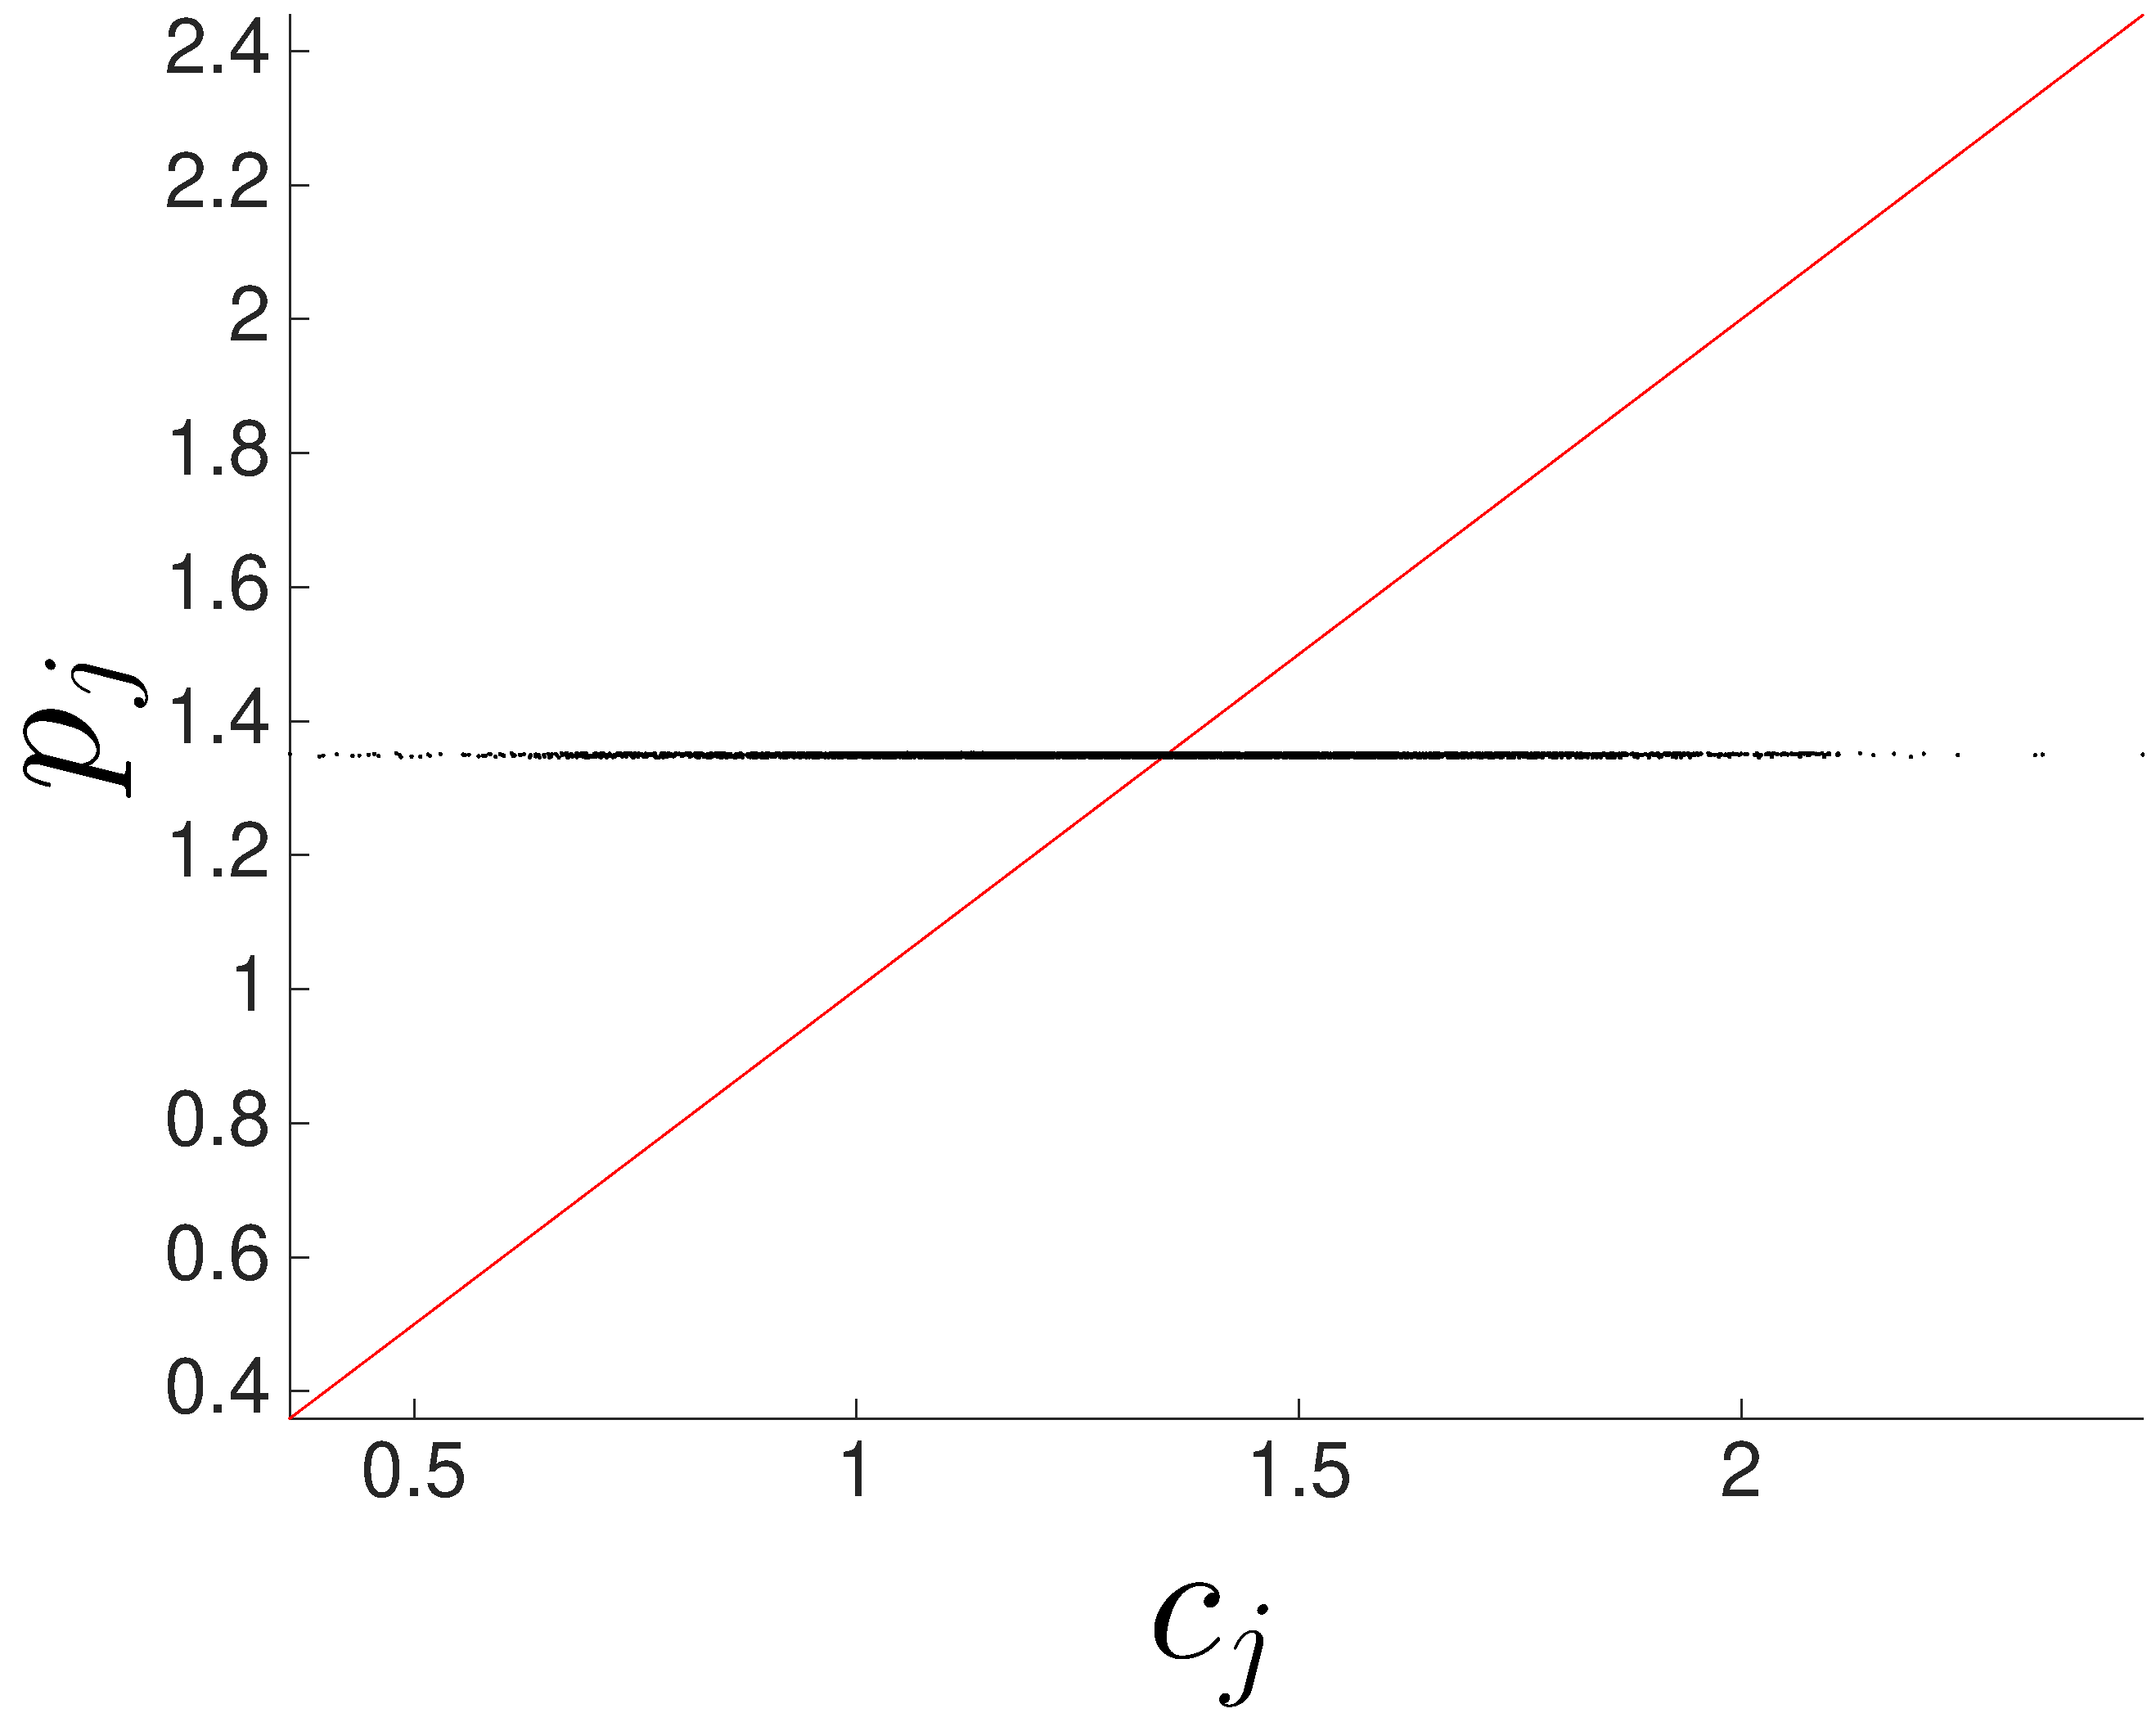
\includegraphics[width=\textwidth]{figs/gccMeanForecast}
    \caption{\gcc na\"ive }
    \label{fig:gccMEAN}
  \end{subfigure}%      
  \\
    \begin{subfigure}{0.49\textwidth}
    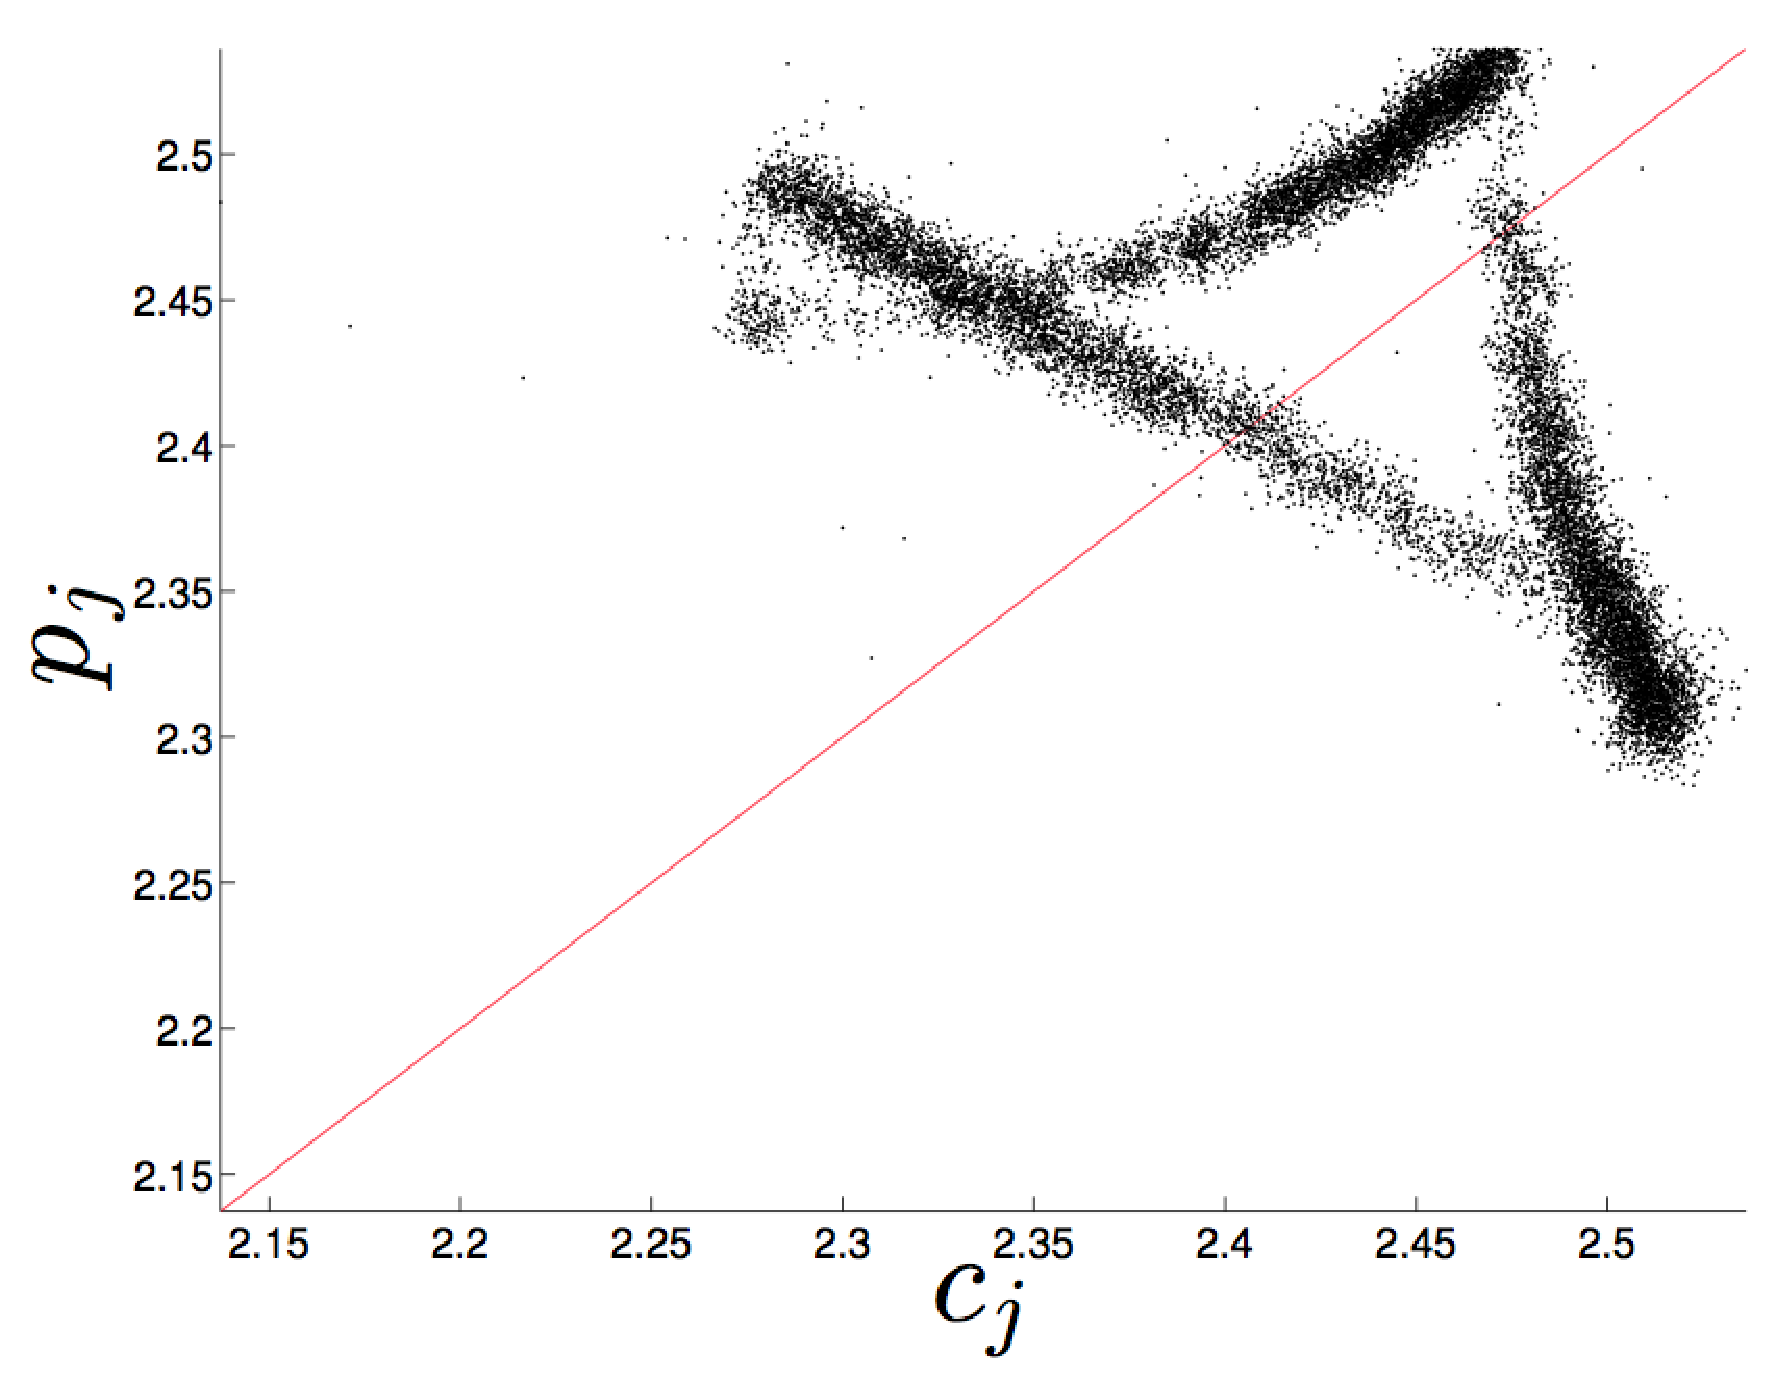
\includegraphics[width=\textwidth]{figs/colARIMAForecast}
    \caption{\col ARIMA}
    \label{fig:colARIMA}
  \end{subfigure}
  \begin{subfigure}{0.49\textwidth}
    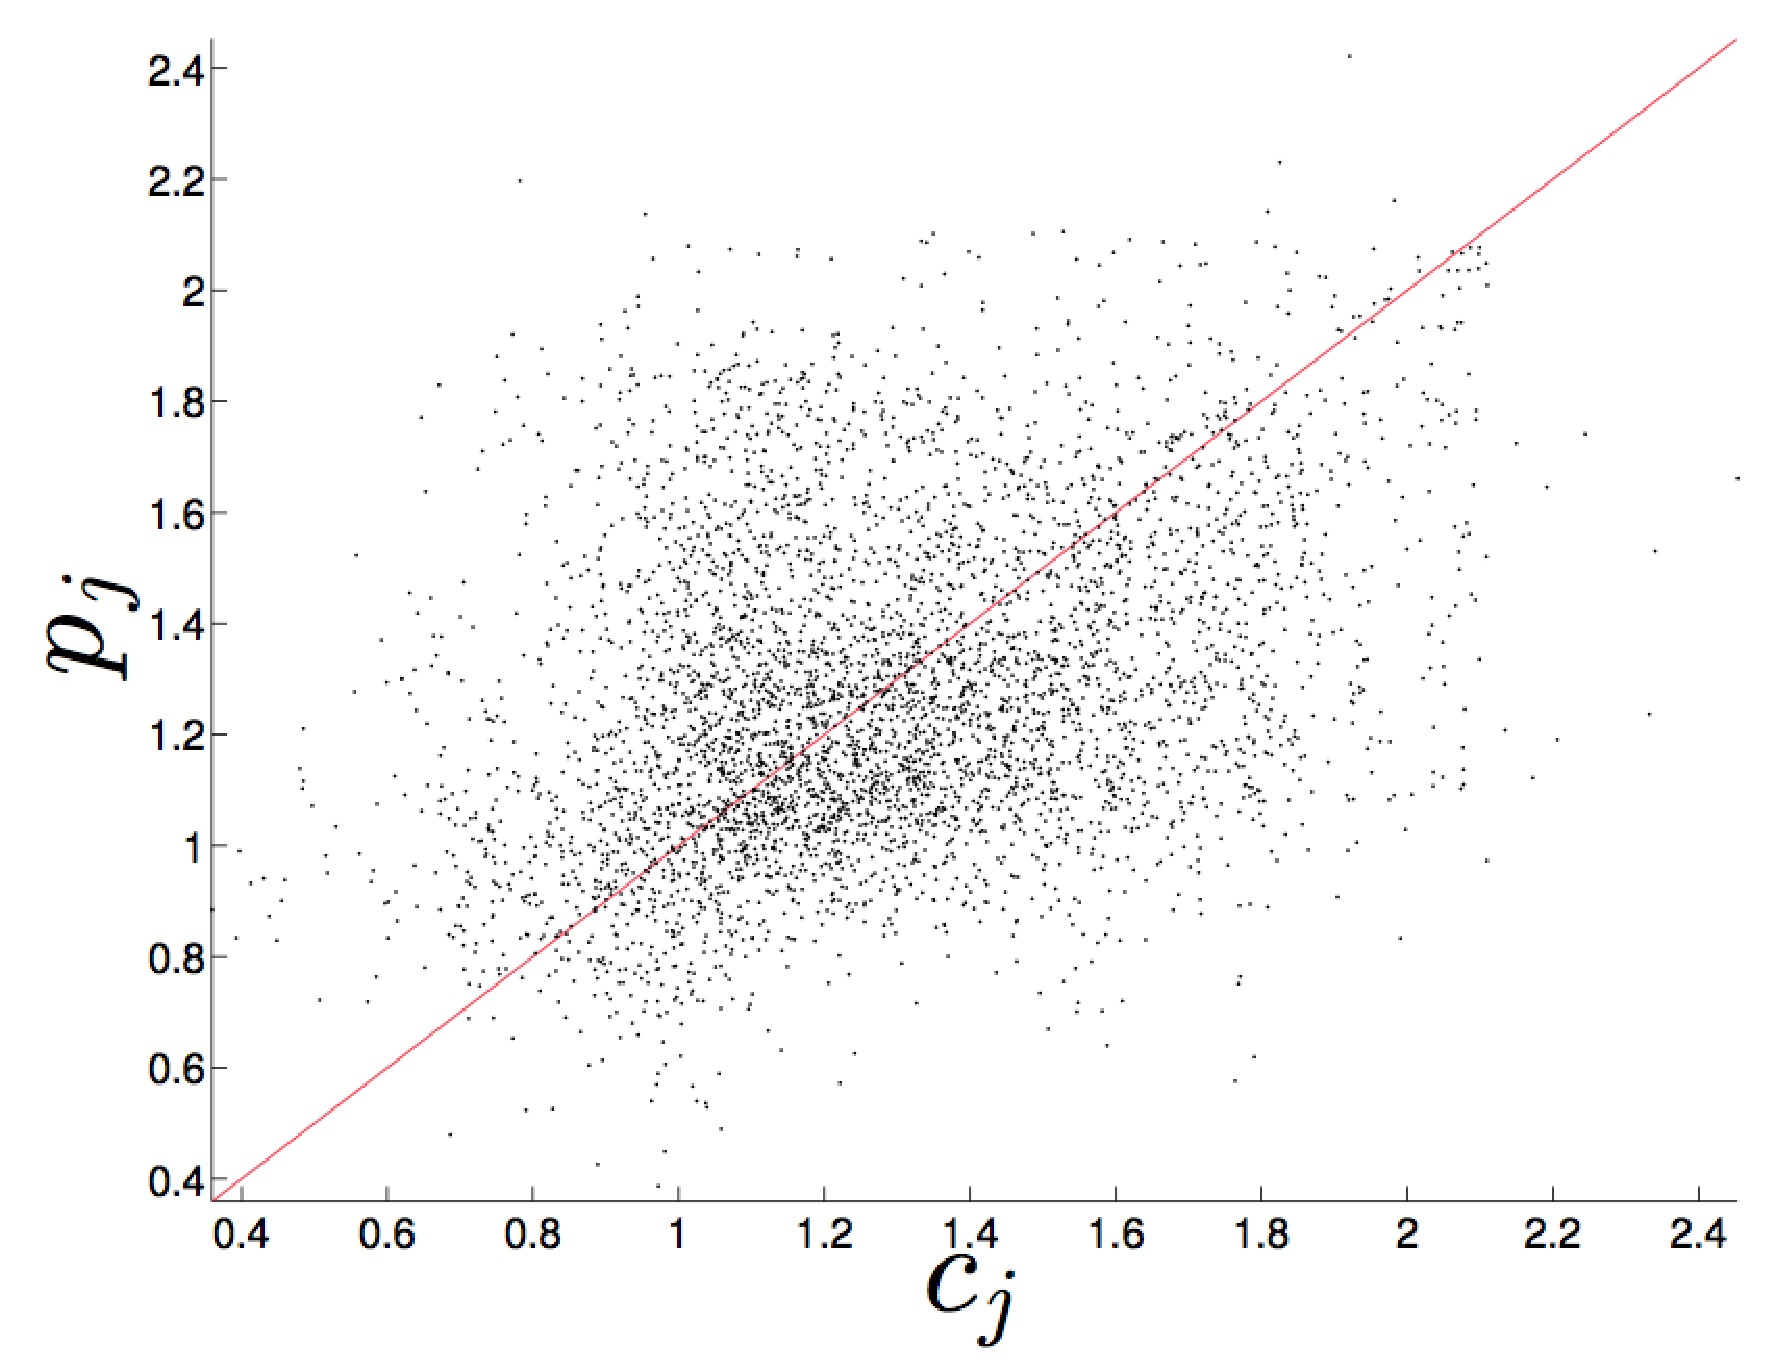
\includegraphics[width=\textwidth]{figs/gccARIMAForecast}
    \caption{\gcc ARIMA }
    \label{fig:gccARIMA}
  \end{subfigure}%
  \\
      \begin{subfigure}{0.49\textwidth}
    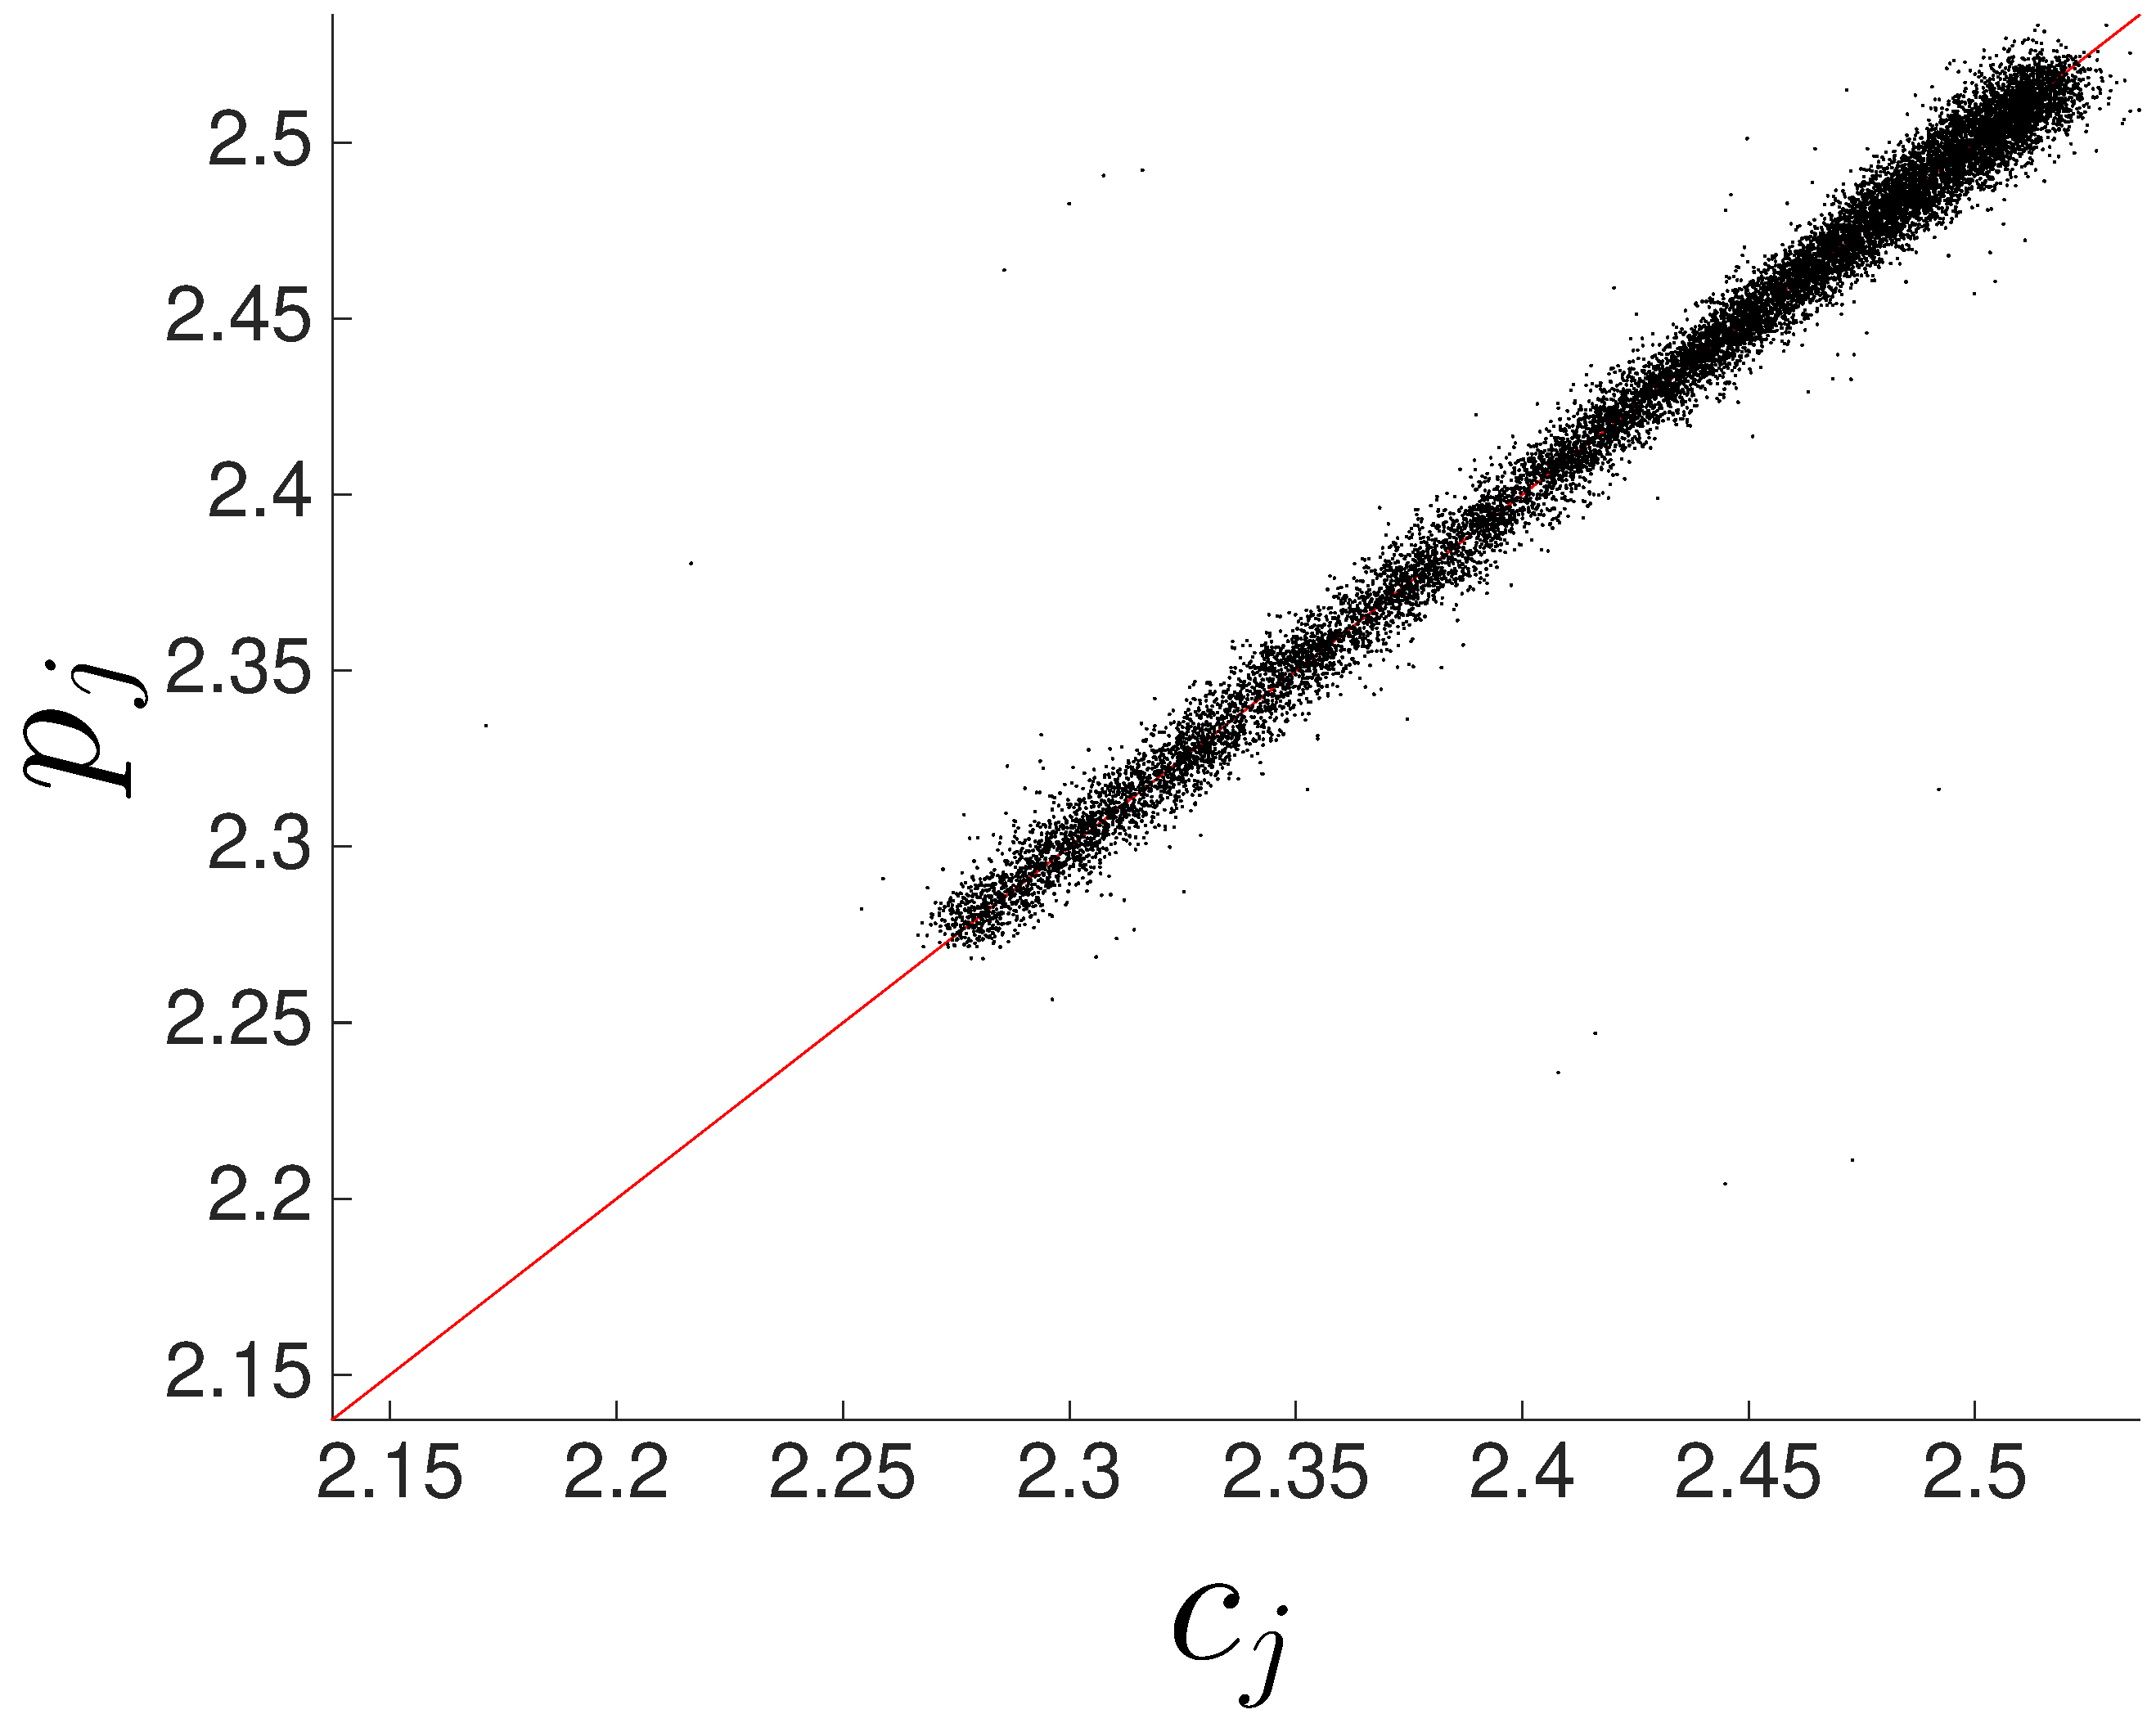
\includegraphics[width=\textwidth]{figs/colLMAForecast}
    \caption{\col LMA}
    \label{fig:colLMA}
  \end{subfigure}
      \begin{subfigure}{0.49\textwidth}
    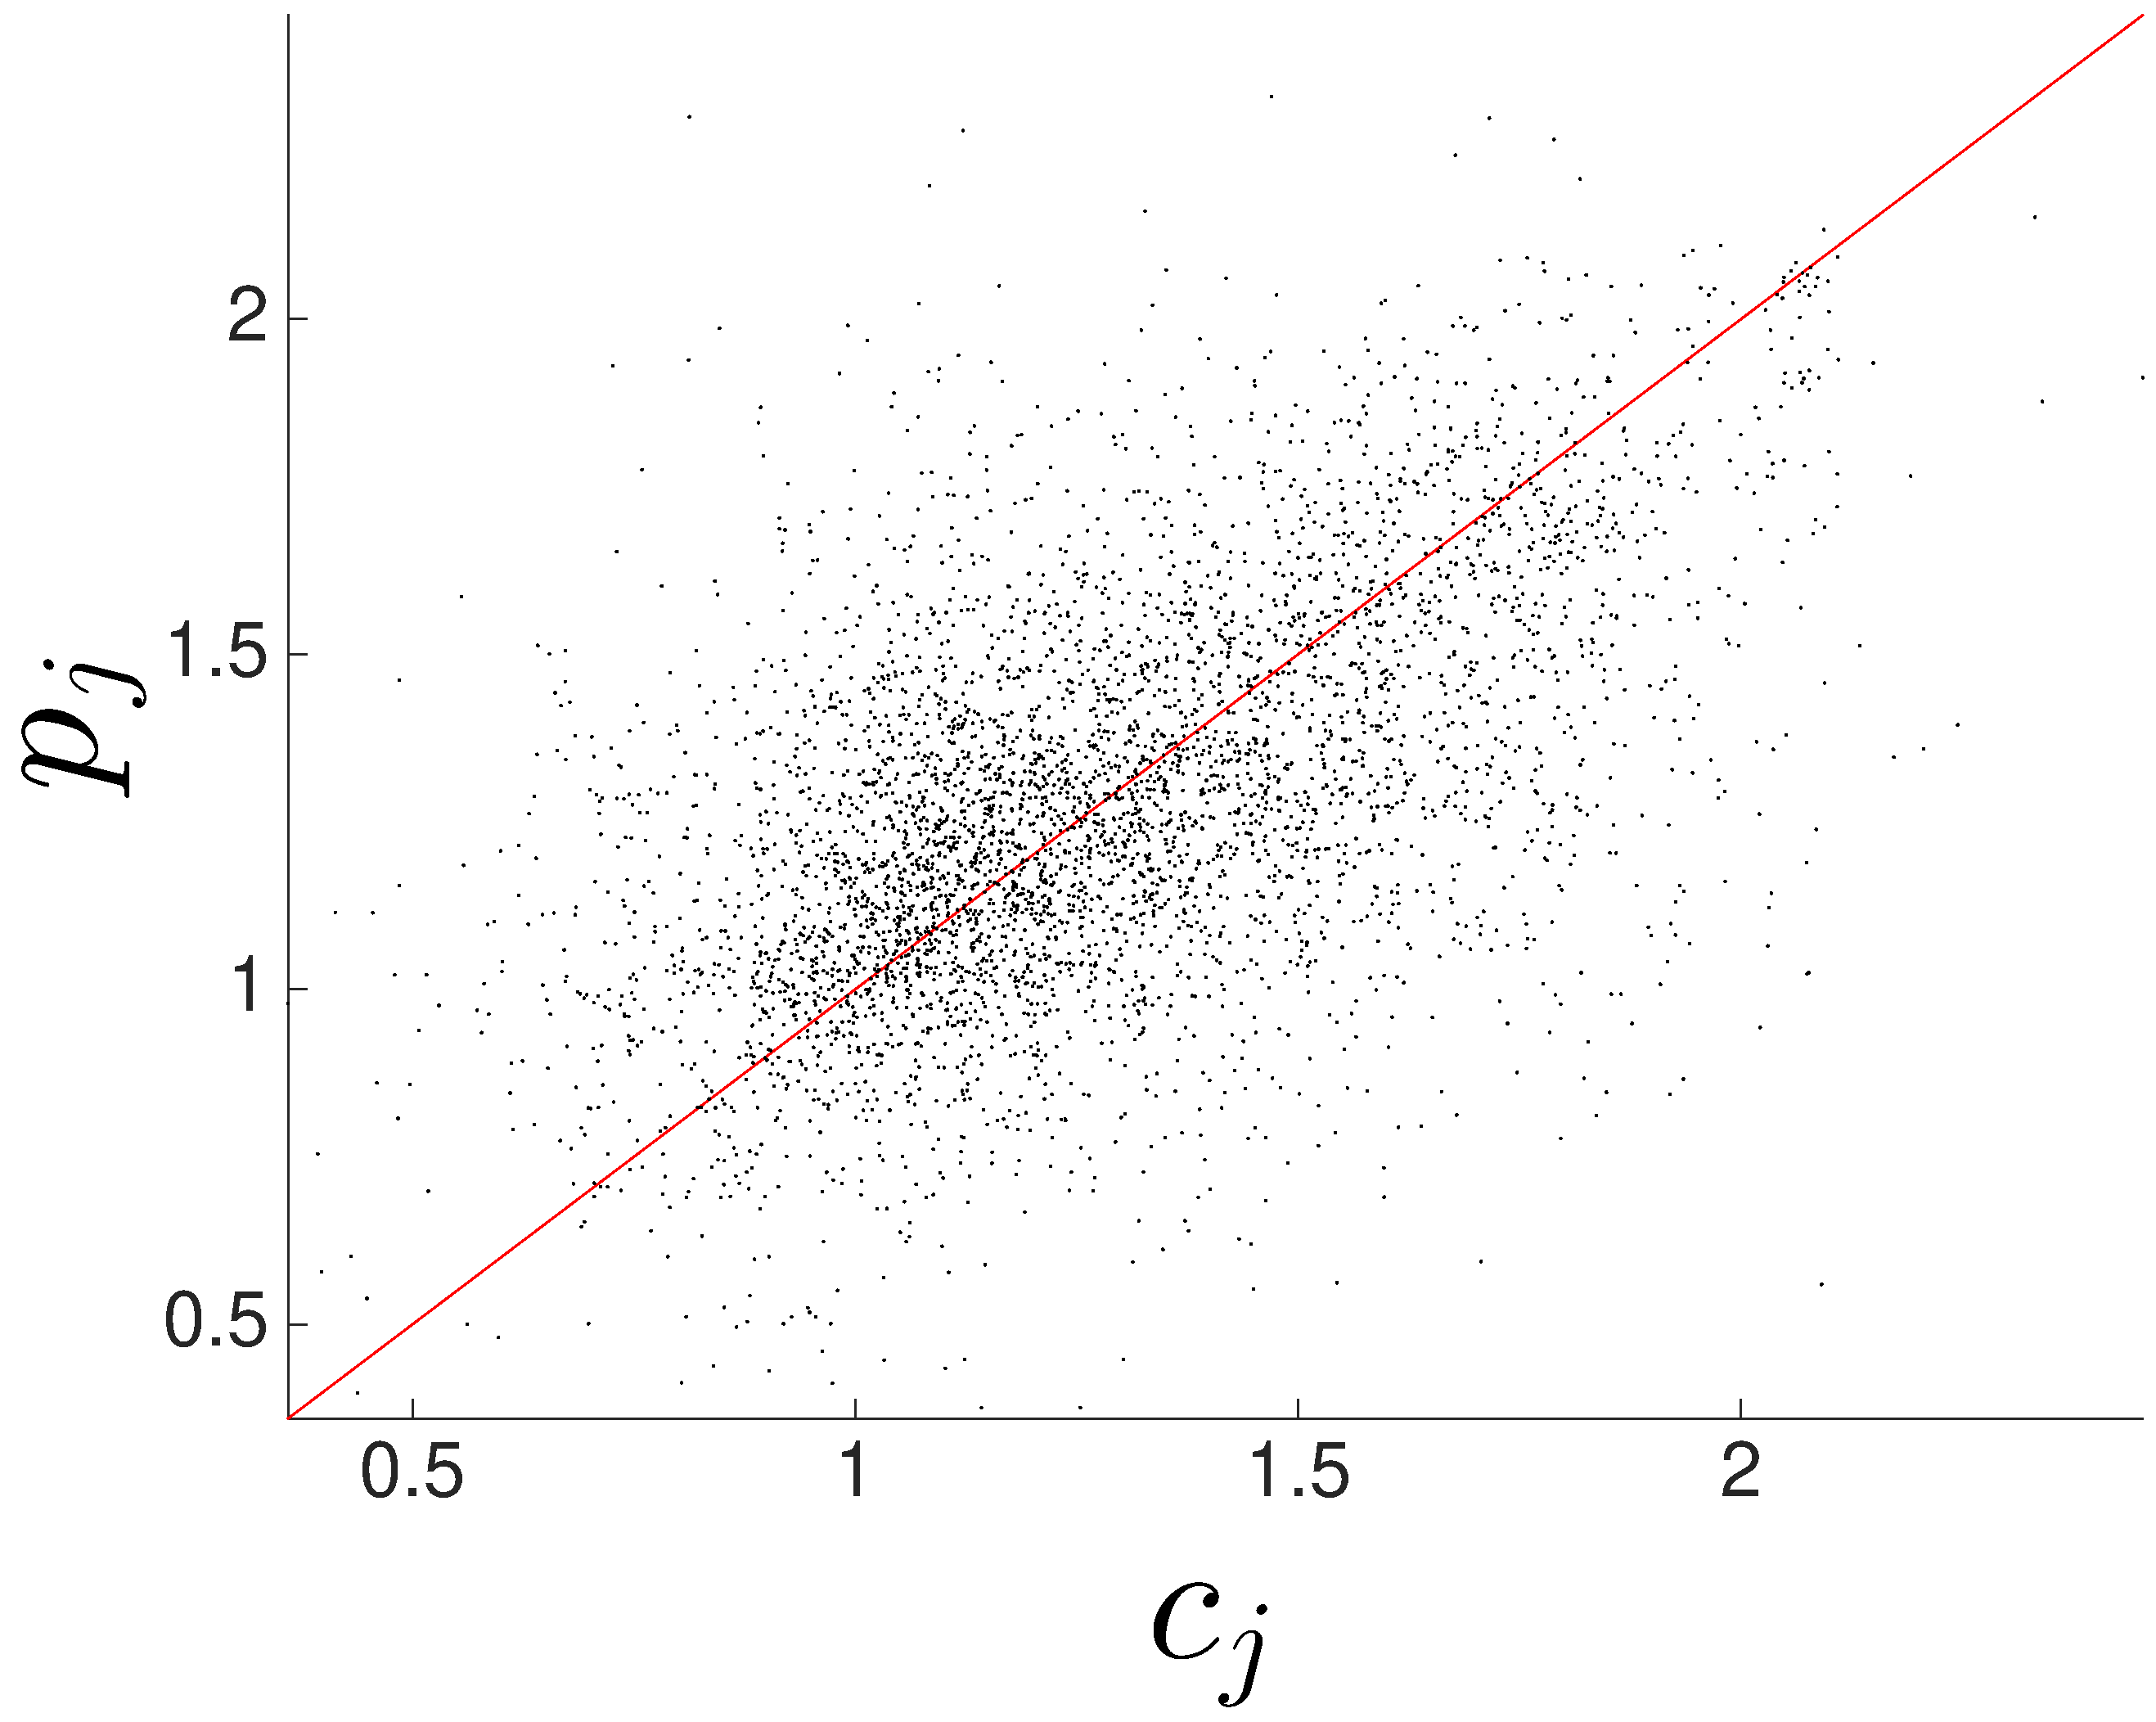
\includegraphics[width=\textwidth]{figs/gccLMAForecast}
    \caption{\gcc LMA}
    \label{fig:gccLMA}
  \end{subfigure}  


  
  %\begin{subfigure}{0.5\textwidth}
  %  \includegraphics[width=1.0\textwidth]{figs/LMA_vs_ARIMA}
   \caption{
For each of these, we plot the predicted value $p_n$ against the correct value $c_n$. On this type of plot a perfect prediction lies exactly on the diagonal, that is the line $p_n = c_n$, e.g., \ref{fig:colLMA} is a near perfect prediction where-as \ref{fig:gccARIMA} is a very poor prediction. }\label{fig:gcc_vs_col}  
  %\end{subfigure}
\end{figure} 
In order to analyze correctness of each prediction we split each time series into two pieces: the first 90\% referred to as the ``learning" or ``training" signal, $\{X_{i,obs}\}_{i=1}^{n}$ and the last 10\% known as the ``test" or ``correct" signal $\{c_j\}_{j=n+1}^{k+n+1}$. The learning signal is used to train an initial model (e.g., LMA or ARIMA) as described in Section \ref{sec:compModel}. The test signal is used both to assess the models forecasting accuracy and for any refitting that may be necessary. In particular, we perform $k$ 1-step predictions, after each 1-step prediction\footnote{We would like to note that this rebuilding occurs due to a problem with ARIMA models converging to a mean prediction if too long of a prediction horizon is used, this is not a handicap of either LMA or na\"ive.} we append the training signal with the next point in the correct signal $c_j$, refit the model taking into account the new system measurement and perform another prediction. This is repeated $k$ times to obtain $\{p_j\}_{j=n+1}^{k+n+1}$.

As a figure of merit we calculate the Mean Absolute Scaled Error (MASE)\cite{MASE} between the true and predicted signals: 
%In order to compare the resulting forecasts we calculate the Mean Absolute Squared Error (MASE)\cite{MASE} between the true and predicted signals:
$$MASE = \sum_{j=n+1}^{k+n+1}\frac{|c_j-p_j| }{\frac{k}{n-1}\sum^n_{i=2}|X_{i,obs}-X_{i-1,obs}|}$$
The scaling term for MASE:
$$\frac{1}{n-1}\sum^n_{i=2}|X_{i,obs}-X_{i-1,obs}|$$ 
is the average in-sample forecast error for a random walk prediction $(p_i=X_{i-1,obs})$. This error method was introduced in \cite{MASE} as a ``generally applicable measurement of forecast accuracy without the problems seen in the other measurements." The major advantage of MASE is that it allows fair comparison across methods, prediction horizons and varying signal scales. When a forecast results in a $MASE<1$ this means that the prediction method gave, on average, smaller errors than the 1-step errors from the in-sample random walk forecast strategy. Analogously, $MASE>1$ means that the prediction method did worse, on average than the 1-step errors for the in-sample random walk forecast strategy. In Table \ref{tab:error} we provide the distribution [[Joshua: Ryan, Is this the right word? we give mean $\pm$ std. dev but some have very skewed right tails]]  of MASEs for each of the 8 signals and 3 prediction strategies, these are averaged over 15 runs of each type (signal + method). [[and cherry pick a few examples of \gcc and \col to put in the text For comparison Table \ref{tab:error} also has the distribution of weighted permutation entropies for word lengths of $l=6$.]]







% took out for space

